\pdfoutput=1
\pdfminorversion=5
\pdfsuppresswarningpagegroup=1
%%%%%%%%%%%%%%%%%%%%%%%%%%%%%%%%%%%%%%%%%%%%%%%%%%%%%%%%%%%%%%%%%%%%%%
%                          template.tex
%
% LaTeX template for papers conforming to the United States Sections of
% the Combustion Institute style guide.
%
% Authors:
%     Bryan W. Weber, University of Connecticut
%     Kyle E. Niemeyer, Oregon State University
%
% This work is licensed under the Creative Commons Attribution 4.0
% International License. To view a copy of this license, visit
% http://creativecommons.org/licenses/by/4.0/.
%
% The source for this template can be found at
% https://github.com/pr-omethe-us/ussci-latex-template
%%%%%%%%%%%%%%%%%%%%%%%%%%%%%%%%%%%%%%%%%%%%%%%%%%%%%%%%%%%%%%%%%%%%%%%
\documentclass[12pt]{ussci}

\usepackage{graphicx}
\usepackage{caption}
\usepackage{subcaption}
\usepackage{amsmath,amsfonts,amssymb}
\usepackage[version=4]{mhchem}

%better printing of numbers
\usepackage[T1]{fontenc}
\usepackage[english]{babel}
\usepackage{csquotes}
\usepackage{textcomp}

\usepackage{siunitx}
\sisetup{group-separator={,},
     detect-all,
     binary-units,
     list-units = single,
     range-units = single,
     tophrase = --,
     per-mode = symbol-or-fraction,
     separate-uncertainty = true,
     list-final-separator = {, and }
%    scientific-notation = fixed
}
\DeclareSIUnit\atm{atm}

%======================================================================
% BibLaTeX and biber (not BibTeX) are used to process the references,
% so these packages must be installed on your system. All configuration
% for the bibliography and citations are done in the ussci.cls file
% Add your bibliography file here, replacing template.bib

%======================================================================
% Replace "Reaction Kinetics" in the line below by your paper topic
\newcommand\papertopic{Reaction Kinetics}
%======================================================================

\graphicspath{{./Figures/}}

\title{ Investigating stiffness detection metrics for chemical kinetics }

\author[1]{Andrew Alferman}
\author[1,*]{Kyle E. Niemeyer}


\affil[1]{School of Mechanical, Industrial, and Manufacturing Engineering\\
		Oregon State University, Corvallis, OR 97331, USA}
\affil[*]{Corresponding author: \email{Kyle.Niemeyer@oregonstate.edu}}


\begin{document}
\maketitle

%====================================================================
\begin{abstract} % not to exceed 200 words

%Abstract should be between 150--200 words and should state briefly the purpose of the research, the principal results and major conclusions. An abstract is often presented separately from the article, so it must be able to stand alone. For this reason, References should be avoided, but if essential, then cite the author(s) and year(s). Also, non-standard or uncommon abbreviations should be avoided, but if essential they must be defined at their first mention in the abstract itself.

Simulations of combustion and reacting flows often encounter stiffness in the equations governing chemical kinetics.
Explicit solvers for these ordinary differential equations offer low computational expense, but typically cannot efficiently handle stiff systems.
In contrast, implicit methods demand greater expense but offer unconditional stability?as a result, most reactive flow solvers rely on these methods by default (other than explicit direct numerical simulation solvers).
However, explicit or stabilized explicit methods can instead be used to reduce the computational expense while remaining stable and accurate if the chemical kinetics systems exhibit low-to-moderate stiffness.
This study investigates metrics for quantifying stiffness, with the goal of identifying one capable of efficiently and robustly determining the appropriate category of integrator required.
%Ensure this order matches the order that we use later on
Methods of measuring the stiffness of chemical kinetics states will be investigated, including stiffness ratio, stiffness index, stiffness indicator, and chemical explosive mode.
%Also include GRI mech 3.0 if data can be obtained by then
These will be applied to simulations of hydrogen/carbon monoxide autoignition using initial conditions representative of realistic turbulent combustion, obtained from partially stirred reactor simulations.
% Change this to reflect the time needed to integrate explicit methods
The stiffness quantification metrics will be compared with the time required to integrate using implicit methods, and the maximum allowable time step using explicit methods.
We will conclude with preliminary performance analysis of an integrator scheduler using these metrics.

%Literature on stiffness quantification will be surveyed and methods of measuring the stiffness of chemical kinetics states will be investigated, including methods based on eigendecomposition or the spectral radius of the Jacobian matrix, error estimations, conditioning parameters, and computational cost estimations.
%These methods will be applied during the solution of hydrogen and carbon monoxide autoignition with different initial conditions based on partially stirred reactor simulation sampling, and evaluated in terms of effectiveness and computational efficiency.

\end{abstract}

% Provide 2-4 keywords describing your research. Only abbreviations firmly
% established in the field may be used. These keywords will be used for
% sessioning/indexing purposes. Use \sep between each keyword.
\begin{keyword}
    Stiffness quantification\sep Ordinary differential equations\sep Chemical kinetics\sep Computational cost reduction
\end{keyword}

%====================================================================
\section{Introduction}
%

An increasing demand for greater efficiency and lower \ce{CO2} emissions in the US energy supply has driven the development of next-generation combustion technologies that use alternative fuels \cite{Epstein2012}.
Computational modeling is one important tool that increasingly drives design and development of these new technologies.
Shortening the design cycle and time-to-market of novel and efficient energy devices optimized for alternative fuels requires fundamental advances in combustion science and fuel chemistry; both depend on high-fidelity computational tools~\cite{Niemeyer}.
The need to develop new, high-performance computational methods to support combustion research has been recognized by multiple federal agencies as a key objective towards implementing predictive models~\cite{Trouve:2006tq,DOE:2007tj,NationalResearchCouncil:2011ub,National-Research-Council:2014aa}.

Species time scales can range from the order of nanoseconds to seconds, requiring greater computational expense for integration by conventional methods (i.e., numerical stiffness)~\cite{Lu2009}.
Most combustion modeling approaches rely on a single, implicit ODE integration method to handle the chemistry in all spatial locations, but these methods are computationally expensive, especially for larger mechanisms.
The computational cost of chemistry is either a quadratic or cubic function of the number of species~\cite{Lu2009}; reaction mechanisms of sizes comparable to those shown above pose computational difficulties even in zero-dimensional (homogeneous) simulations.

Depending on the local conditions, computational fluid dynamics flow time-step size, and chemical mechanism being used, it is possible to encounter a wide range of stiffness within a single simulation.
We can exploit this situation to reduce the overall simulation expense by selecting the most computationally efficient ODE solver on-the-fly based on local conditions.
For example, a low-cost explicit method may be used far away from the reaction zone, while an implicit---or otherwise ``stiff''---solver is more economical inside a flame.
Making this selection requires a method to detect and classify stiffness~\cite{Niemeyer}.

Although the concept of stiffness has been identified for over 60 years, the term has not been precisely defined despite repeated efforts.
The diverse set of problems considered to be ``stiff'' and the large variety of characterizations used to describe stiffness are amongst the difficulties that have been encountered in developing a precise definition~\cite{Soderlind2014}.
Nonetheless, a variety of stiffness quantification methods have been developed with the goal of providing a practical means of evaluating a systems ODEs~\cite{Soderlind2014,Shampine1985,Brugnano2011,Lambert1973ComputationalEquations,Hairer1996SolvingII}.
We look to these methods of stiffness quantification to determine their usefulness with respect to the equations governing combustion, and to determine if a reliable and efficient means of switching methods can be developed from it.
In doing so, we hope to reduce the computational expense of combustion simulations.

One method of interest regarding stiffness quantification was the ``IA-Stiffness Index'' proposed by Shampine~\cite{Shampine1982}.
This method enables comparison of values of the stiffness index between different equations and different methods.
Additionally, the method takes into account the impact of the order of the method selected when evaluating the stiffness.
The method is relatively straightforward to implement, requiring computation of a vector of the derivatives of the system of equations, as well as either a weighted norm or the spectral radius of the Jacobian matrix.

\section{Methods}
% NEEDS UPDATE
We started using the relatively small hydrogen\slash carbon monoxide (\ce{H2}\slash \ce{CO}) model of Burke et al.~\cite{Burke:2011fh} for our initial investigation into stiffness quantification.
This system only involves 13 chemical species, and therefore the Jacobian matrix need only be $14\times14$ after the temperature derivatives are included.
This small Jacobian matrix allows for much faster evaluations of stiffness than would be possible with larger, more complicated kinetic systems, which can have hundreds to hundreds of thousands of chemical species~\cite{Niemeyer:2013}.
% The stiffness quantification methods investigated using the \ce{H2}\slash \ce{CO} system can easily be applied to more complicated models.

% Something about the stiffer GRI mech 3.0

%Review this sentence
Our analysis was conducted using information gathered from partially stirred reactor (PaSR) simulations.
As described by Niemeyer et al.~\cite{Niemeyer:2017}, the PaSR model consists of a number of particles, each with a time-varying composition.
At discrete time steps, events including inflow, outflow, and pairing cause particles to change composition; between these time steps, mixing and reaction fractional steps evolve the composition of all particles.
By using data from a single particle at a single time step of the PaSR model, the evaluation could be simplified to a zero-dimensional analysis.
%Update this sentence
The stiffness detection metrics and method-switching algorithm developed in the zero-dimensional analysis may be applied to more complicated models in future work.
(Please refer to Niemeyer et al.~\cite{Niemeyer:2017} for a detailed description of the relevant equations and solution technique.)



The IA-stiffness index of a method of order \textit{p} introduced by Shampine~\cite{Shampine1982} is
\begin{equation}
    \frac{h_{acc}}{h_{iter}} \doteq \tau ^ {1/(p + 1)} \rho [f_y(x_n,y(x_n))] \|y^{(p+1)}(x_n)\|^{-1/(p+1)} \left( \frac{|\xi|^{-1/(p+1)}}{|\gamma|} \right)
\end{equation}
or alternatively,
\begin{equation}
    \frac{h_{acc}}{h_{iter}} \doteq \tau ^ {1/(p + 1)} \|f_y(x_n,y(x_n))\|\|y^{(p+1)}(x_n)\|^{-1/(p+1)} \left( \frac{|\xi|^{-1/(p+1)}}{|\gamma|} \right)
\end{equation}
where $h_{acc}$ represents the largest step size which would result in a local accuracy test being passed, $h_{iter}$ represents the minimum step size that will lead to divergence of simple iteration, $\tau$ represents the specified tolerance, $\rho [f_y(x_n,y(x_n))]$ represents the spectral radius of the Jacobian matrix $f_y(x_n,y(x_n))$, $\gamma$ is a constant characteristic of the formula, and $\xi$ represents a constant characterizing the accuracy of a reference method.
Note that these equations require the $p+1$ derivative of the function $y(x_n)$.
Additionally, the matrix norm $\|M\|$ of matrix $M$ with $i$ columns and $j$ rows is given by
\begin{equation}
    \|M\| = \max_{i} \frac{1}{w_i} \sum_{j} |M_{ij}|w_j
\end{equation}
in which \(w_i\) and \(w_j\) are positive weights of the matrix~\cite{Shampine1985}.

Although the IA-stiffness index is useful in determining the stiffness of a method for a given system of equations, we are interested in quantifying the stiffness inherent to the system of equations itself.
Such a quantification is necessary for investigating method switching mechanisms.
Shampine notes that the scalar quantity
\begin{equation}\label{eqn:stiffness}
    \textrm{index} = \rho [f_y(x_n,y(x_n))] \|y^{(p+1)}(x_n)\|^{-1/(p+1)}
\end{equation}
provides a fair ``stiffness index'' to a given problem~\cite{Shampine1985}. For the remainder of this document, all references to the stiffness index will refer to the value obtained using equation (\ref{eqn:stiffness}).

% Stiffness indicator discussion

As previously noted, use of the above equations requires calculation of a vector of the derivatives of a system of equations.
In the case of this investigation, this vector is comprised of the derivatives of the thermochemical composition vector with respect to time, with the the vector defined as
\begin{equation}
    \Phi = \{T, Y_1, Y_2, \dots, Y_{N_{sp}} \}^\intercal \;,
\end{equation}
where $T$ is the temperature, $Y_i$ are the species mass fractions, and $N_{sp}$ is the number of species in the mechanism~\cite{Niemeyer:2017}.
The vector needed to compute the stiffness index is therefore
\begin{equation}
    \frac{\partial \Phi}{\partial t} = \left\{\frac{\partial Y_1}{\partial t}, \frac{\partial Y_2}{\partial t}, \dots, \frac{\partial Y_{N_{sp}}}{\partial t} \right\}^\intercal \;,
\end{equation}
where time is denoted by $t$~\cite{Niemeyer:2017}.
In addition to this vector of derivatives, computation of the stiffness index requires either the weighted norm or the spectral radius of the Jacobian matrix for the thermochemical composition vector.
Computation of the vector of derivatives and the Jacobian matrix was readily achieved using pyJac~\cite{pyJac:1.0.2}, a Python-based open-source program that generates analytical Jacobian matrices for use in chemical kinetics modeling and analysis~\cite{Niemeyer:2017}.
pyJac uses a chemical mechanism developed using Cantera~\cite{Goodwin:2015aa} software and a set of initial conditions to generate functions that return the required values.
After generating this data using pyJac, the values of the second derivative of the thermochemical composition vector were calculated numerically using a fourth-order central differencing formula.
Higher-level derivatives may also be generated using the same numerical approach.
Use of the central differencing formula was possible because the stiffness index was calculated after solving for the thermochemical composition vector, and the reaction was modeled using time steps of a constant size.
Forward and backward difference formulae were used at the boundaries where central differencing could not be used.
Variable time step methods for calculating the second derivative or higher-level derivatives may also be used, however these methods were not necessary at the current stage of the investigation.

The code used to calculate the stiffness index was written in Python and made use of open-source software including the \texttt{odeint} integrator function of SciPy~\cite{SciPy}.
This integrator uses the LSODA solver from the FORTRAN library \texttt{odepack} \cite{A.C.Hindmarsh1983}, which incidentally has its own algorithm for automatically switching between a non-stiff and a stiff solver.
To ensure a high degree of accuracy, the integrator was given values of \num{e-13} and \num{e-15} for the error control parameters \texttt{relerr} and \texttt{abserr}, respectively.
\texttt{NumPy}~\cite{VanDerWalt2011} was also extensively used in the code to calculate the stiffness index.
At the current stage of this investigation, the selection of the integrator has no impact on the evaluation of the stiffness index due to the a posteriori approach.
Rather than determining the higher-level derivatives based on the order of the solver used, the order of the method is manually entered into the code.
To facilitate comparison of the results obtained by Shampine~\cite{Shampine1985}, the order of the method was assumed to be 1.
To ensure that the code was running properly, the van der Pol equation with a \(\epsilon\) value of 1000 was used as a test equation.

\section{Results and Discussion}
%
The initial condition of the evaluation was taken from a particle and time in the PaSR simulation, where weak reactions were taking place but ignition had not yet occurred.
A 0.5 second simulation was run by integrating the derivative vector function.
Data obtained from the integration demonstrates that autoignition was achieved with a residence time of approximately 0.11 seconds.
The initial temperature of the simulation was approximately \SI{865}{\kelvin}, which rapidly increases to \SI{2440}{\kelvin} within \SI{0.001}{\second} (i.e., autoignition).
After ignition, the temperature remains nearly constant for the remainder of the simulation. The mass fractions of all of the species considered in the model exhibited similar trends; each rapidly changing then becoming nearly constant immediately after ignition.
The data obtained from the integration was then used to compute the stiffness index for every time step of the integration.

To minimize the computational expense of determining the stiffness index of a given mechanism, a solver can be modified to compute the index at the same time that it calculates values of the solution.
The algorithm would then maximize the use of values already computed to provide the solution value, which makes it most desirable for use with algorithms making use of Jacobian matrices and values of the time derivatives.

\subsection{Results}

%\begin{figure}[htbp]
%    \centering
%    \begin{subfigure}{0.43\textwidth}
%        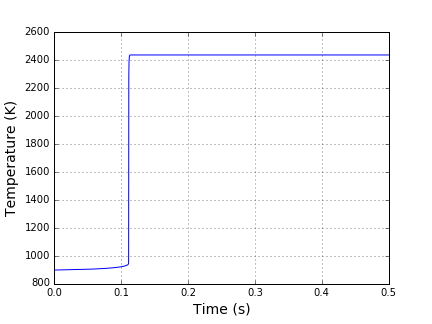
\includegraphics[width=\linewidth]{IndexVals_1e-07_temp.png}
%        \caption{Temperature, 0.0 to 0.5 seconds}
%        \label{fig:tempcurve0}
%    \end{subfigure}
%    \begin{subfigure}{0.43\textwidth}
%        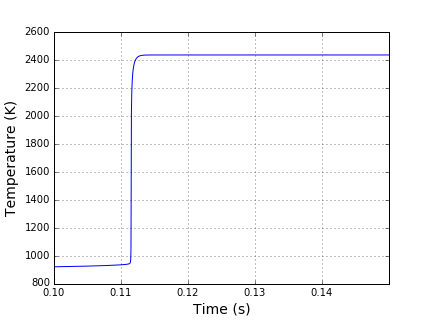
\includegraphics[width=\linewidth]{IndexVals_1e-07_temp_1.png}
%        \caption{Temperature, zoomed \SIrange{0.1}{0.15}{\second}}
%        \label{fig:tempcurve1}
%    \end{subfigure}
%    \begin{subfigure}{0.43\textwidth}
%        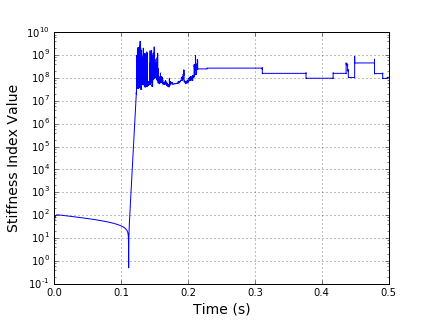
\includegraphics[width=\linewidth]{IndexVals_1e-07_0.png}
%        \caption{Stiffness index, order 1, \SIrange{0.0}{0.5}{\second}}
%        \label{fig:stiff0}
%    \end{subfigure}
%    \begin{subfigure}{0.43\textwidth}
%        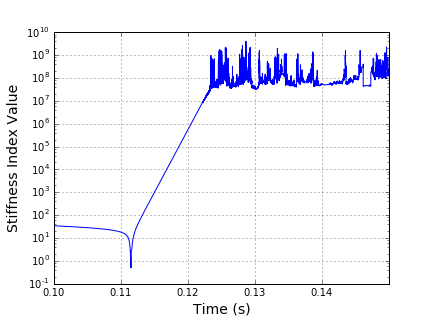
\includegraphics[width=\linewidth]{IndexVals_1e-07_1.png}
%        \caption{Stiffness index, order 1, zoomed \SIrange{0.1}{0.15}{\second}}
%        \label{fig:stiff1}
%    \end{subfigure}
%        \begin{subfigure}{0.43\textwidth}
%        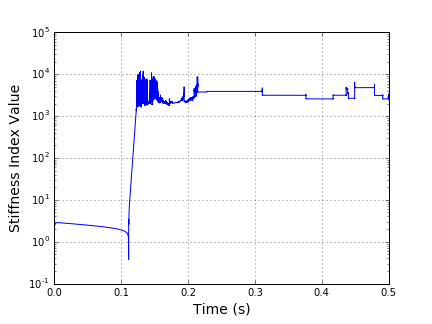
\includegraphics[width=\linewidth]{IndexVals_Order5_1e-07_O5_2.png}
%        \caption{Stiffness index, order 4, \SIrange{0.0}{0.5}{\second}}
%        \label{fig:stifforder4}
%    \end{subfigure}
%    \caption{Temperature and stiffness index of the reaction calculated with a constant step size of \SI{e-7}{\second}.
%    The stiffness index reached its maximum values after \SI{0.12}{\second} when the temperature of the reaction had already stabilized.}
%    \label{fig:initialdata}
%\end{figure}

Values of the stiffness index varied between \num{e-1} and \num{e10} throughout the evaluation.
The stiffness index of the reaction was greatest a short time after the reaction had stabilized following ignition, with values on the order of \numrange{e9}{e10}.
For comparison, the maximum stiffness index for the van der Pol equation with $\epsilon = 1000$, which is considered to be a ``stiff'' equation, is between \numrange{e4}{e5}~\cite{Shampine1985}.
Figure~\ref{fig:initialdata} compares the value of the temperature and stiffness index of the simulation.
Figures \ref{fig:tempcurve0} and \ref{fig:stiff0} show the temperature and stiffness index respectively of a method of order 1 across the full 0.5 second range of the simulation.
Figures \ref{fig:tempcurve1} and \ref{fig:stiff1} also show the temperature and stiffness index respectively of a method of order 1 but are stretched from 0.1 to 0.15 seconds of the simulation to show greater detail immediately before and after autoignition.
Figure \ref{fig:stifforder4} demonstrates the reduction in stiffness due to an increase in order of the method to order 4.

The value of the stiffness index at the start of the evaluation was approximately \num{e2}.
The stiffness index reached a minimum value of slightly less than 1 right as autoignition began.
During the residence time, the index decreased by one order of magnitude.
After spiking at its minimum value of less than 1, the stiffness index rapidly increased until reaching values between \numrange{e7}{e10}.
The stiffness index values obtained have visually apparent noise after reaching the maximum values, even with a step size as small as \num{e-7}.
Although further refinement of the step size and integration tolerance may reduce the magnitude of this noise to some extent, the values remained relatively consistent within the range of \numrange{e7}{e10}.

Furthermore, the stiffness index decreased substantially when the order of the method was increased to four.
While the stiffness index exhibited many of the same trends as before, the maximum stiffness index ranged between \numrange{e3}{e4}.

\section{Conclusions}
%
Our analysis demonstrated that the stiffness of the model prior to autoignition increases significantly during and after autoignition.
This observation matches the expected behavior based on our intuition of the problem, but is based on a calculated metric.
It also demonstrates the feasibility of using an explicit method prior to autoignition to save computational expense.
Interestingly, we did not observe the maximum value of stiffness index during ignition; instead, this value occurred around \SI{0.02}{\second} after the reaching equilibrium (i.e., steady-state temperature and mass fractions).
After reaching its maximum value, the stiffness remained relatively constant.
The stiffness index evaluated provides a reasonable means of detecting the stiffness of combustion reactions.
Incorporating calculation of this index in the code used to integrate the derivative vector will both accelerate calculation of the index and enable the index to be calculated on-the-fly.

\section{Acknowledgements}
This material is based upon work supported by the National Science Foundation under grant ACI-1535065.

\bibliographystyle{elsarticle-num}
\bibliography{ConfPaper.bib}
\bibliography{mendeley.bib}


\end{document}
